% Requires graphicx. Copy the PDF beside this fragment or adapt its path.
% Figure number 10 is assigned by the surrounding report's figure counter.
\begin{figure}[htbp]
    \centering
    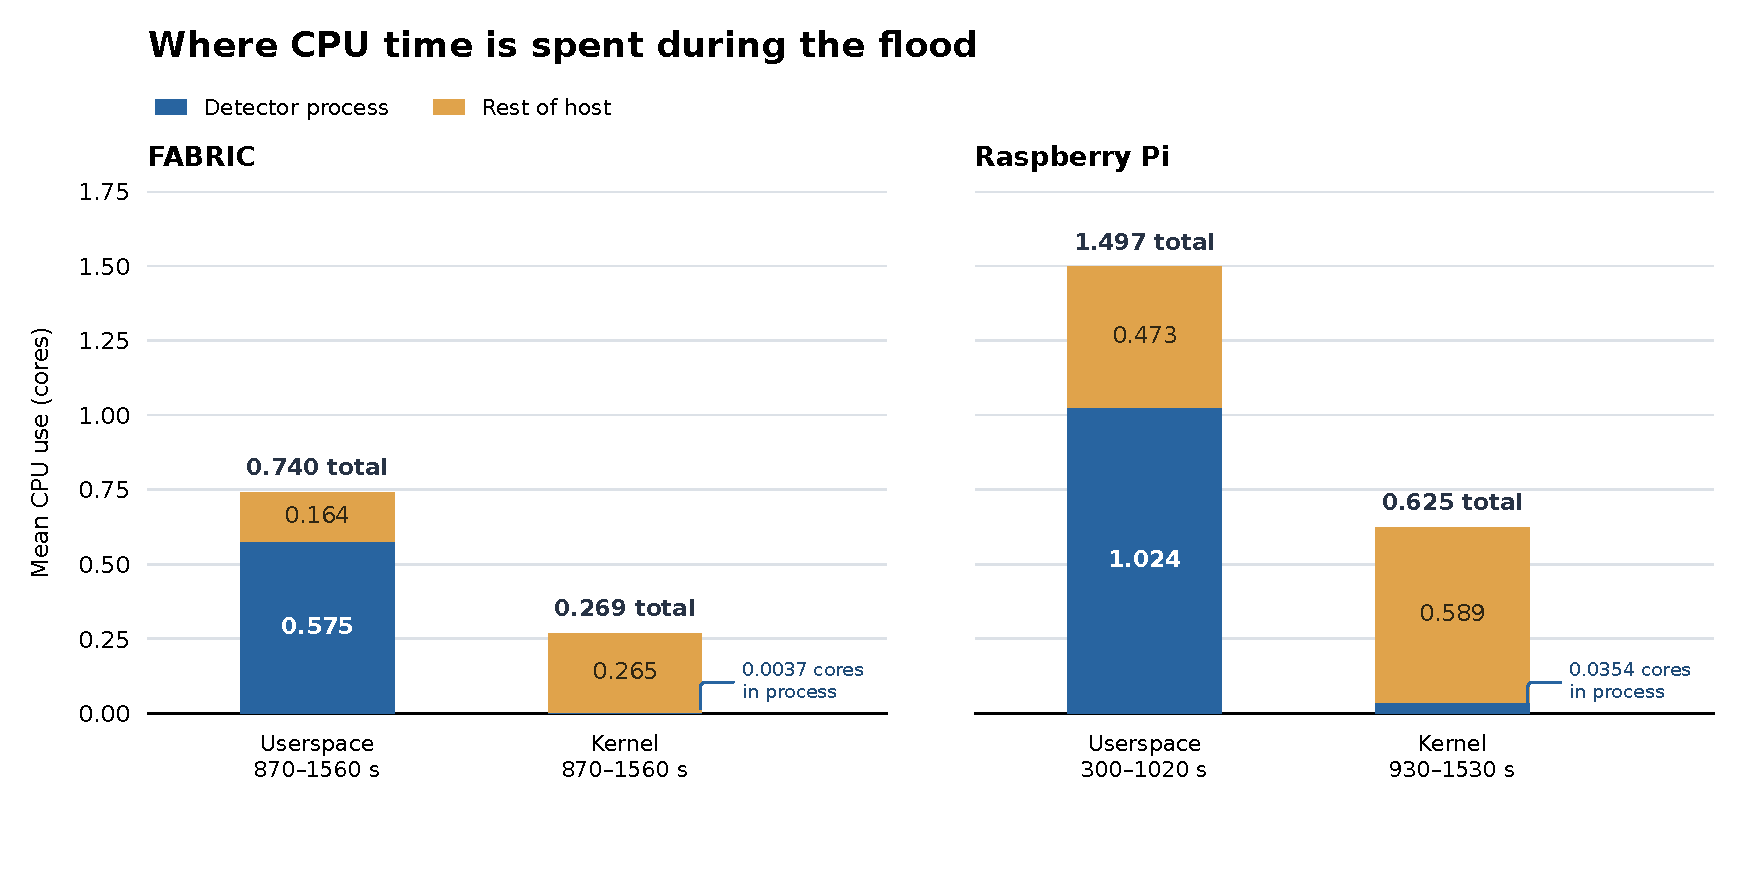
\includegraphics[width=\linewidth]{figure-10-cpu-breakdown.pdf}
    \caption{Where CPU time is spent during the flood, with blocking disabled.
    FABRIC and Raspberry Pi recordings are summarized over independently
    selected high-rate phases; each bar represents one recording. Phase
    intervals are shown on each recording's local clock. The selection uses
    the longest span of 30-second traffic bins above half the recording's
    95th-percentile binned packet rate, with one bin trimmed at each edge.
    Values are mean CPU use in cores, calculated
    from CPU-time deltas divided by measured wall time. The rest-of-host
    segment is whole-host busy time minus detector-process CPU time and
    includes unrelated host activity. In the kernel implementation the
    per-packet XDP work runs in software-interrupt context and is not charged
    to the detector process. Observed traffic rates differ between recordings;
    these are descriptive measurements rather than controlled same-load effects.}
    \label{fig:cpu-time-breakdown}
\end{figure}
